\documentclass[../main.tex]{subfiles}

\setstretch{0.1} % Adjusted to improve document readability

\begin{document}

{\let\clearpage\relax\chapter{Methods and Materials}}
\vspace{-5pt}
\section{Initial Approach Using Ray Tracing in \texttt{C++}}
\vspace{-15pt}
\textbf{Ray tracing} is a rendering technique that simulates the way light interacts with objects to generate images with high visual realism. Unlike rasterization, which is used in most real-time graphics, ray tracing calculates the color of pixels by tracing the path that light would take as it travels through a scene. This path is traced backwards from the viewer's eye to the light source, a method known as \textit{backward ray tracing}.

Initially, the simulation of optical flat measurements was attempted using a ray tracing technique in C++. Ray tracing is a powerful computational method for simulating the path of light through media. It models the propagation of light rays and their interactions with surfaces, which is particularly useful in optical studies where the understanding of light behavior in precise environments is necessary. However, this approach did not yield successful results due to complexities in accurately modeling the intricate interference patterns that are critical in optical flat evaluations.
\vspace{-15pt}
\section{Successful Simulation Using Python}
\vspace{-15pt}
After the initial setbacks, a more successful simulation was developed using Python. This method utilized the concept of intersecting planes with the surface under test (sft) (see figure \ref{fig:planes_intersection}). Each plane was separated by half the wavelength of the light transmitted through the optical flat, allowing for the simulation of interference patterns by modeling how these planes interact with the sft irregularities as can be seen in figure \ref{fig:fringes}.
\vspace{-15pt}
\begin{figure}[H]
    \centering
    \hfill
    \begin{minipage}{0.49\textwidth}
        \centering
        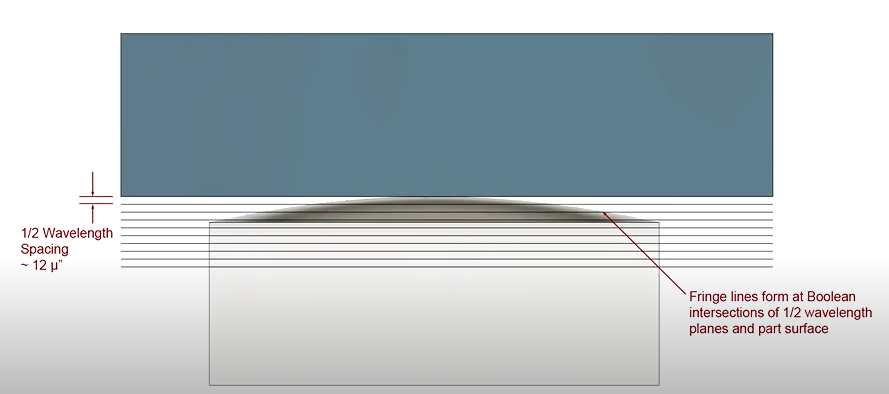
\includegraphics[width=0.95\linewidth]{Images/Methods/planes}
        \caption{
            The blue area at the top represents an optical flat placed over a test surface shown in grey. The white lines, spaced half a wavelength apart, are interference fringes. These fringes form at points where the height difference between the optical flat and the surface matches multiples of half the light's wavelength. The pattern of these fringes reveals the topography of the surface beneath the flat. Figure taken from \cite{youtube}.}
        \label{fig:planes_intersection}
    \end{minipage}
    \hfill
    \begin{minipage}{0.49\textwidth}
        \centering
        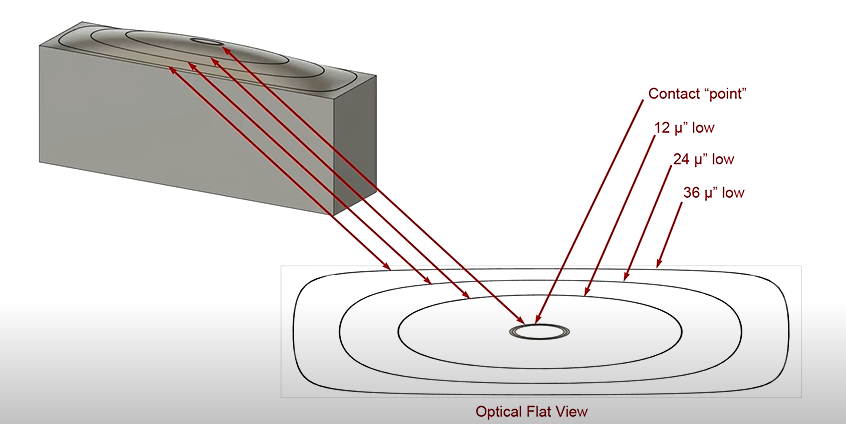
\includegraphics[width=1\linewidth]{Images/Methods/planes_fringee}
        \caption{A 3D model with an optical flat above a test surface and a 2D projection. Red lines represent light rays reflecting at different gaps between the optical flat and the surface. These variations are visible in the 2D "Optical Flat View" as concentric circular fringes, each indicating a constant air gap. This method precisely measures the deviations in surface flatness, with each ring in the diagram quantifying specific irregularities. Figure taken from \cite{youtube}.}
        \label{fig:fringes}
    \end{minipage}
\end{figure}
\vspace{-35pt}
\subsection{Backend Development: Python Scripts}
\vspace{-10pt}
To implement this method, several Python scripts were created:
\vspace{-4pt}
\begin{itemize}
    \setlength{\itemsep}{0.1mm}
    \item \textbf{Intersection} - This function, as can be seen in figure \ref{fig:flowchart1}, handles the mathematical computation of plane and surface intersections, critical for modeling how light interacts with different surfaces.
    \item \textbf{Disk, Cylinder, Flat\_surface, Shape3D, STLFigure} - These classes contribute to generating and handling various geometrical shapes and rendering the final 3D images which represent the simulation results.
\end{itemize}

\tikzstyle{startstop} = [rectangle, rounded corners, minimum width=1cm, minimum height=1cm,text centered, draw=black, fill=red!30, font=\scriptsize]
\tikzstyle{io} = [trapezium, trapezium left angle=70, trapezium right angle=110, minimum width=3cm, minimum height=1cm, text centered, draw=black, fill=blue!30]
\tikzstyle{process} = [rectangle, minimum width=3cm, minimum height=1cm, text centered, draw=black, fill=orange!30]
\tikzstyle{decision} = [diamond, minimum width=3cm, minimum height=1cm, text centered, draw=black, fill=green!30]
\tikzstyle{arrow} = [thick,->,>=stealth]
\vspace{-8pt}

\begin{figure}[H]
    \centering
    \begin{tikzpicture}[scale=0.75, transform shape, node distance=1cm, auto]
    % Styles for flowchart elements
    \tikzstyle{startstop} = [rectangle, rounded corners, minimum width=0.5cm, minimum height=0.5cm,text centered, draw=black, fill=red!30, font=\footnotesize]
    \tikzstyle{io} = [trapezium, trapezium left angle=70, trapezium right angle=110, minimum width=0.5cm, minimum height=0.5cm, text centered, draw=black, fill=blue!30, font=\footnotesize]
    \tikzstyle{process} = [rectangle, minimum width=0.5cm, minimum height=0.5cm, text centered, draw=black, fill=orange!30, font=\footnotesize]
    \tikzstyle{decision} = [diamond, minimum width=0.5cm, minimum height=0.2cm, text centered, draw=black, fill=green!30, font=\footnotesize]
    \tikzstyle{arrow} = [thick,->,>=stealth]
    
    % Nodes
    \node (start) [startstop, xshift=-4cm] {Start};
    \node (in1) [io, below of=start, yshift=-1cm] {Input: shape1, shape2};
    \node (pro1) [process, below of=in1, yshift=-1cm] {Get surface points for both shapes};

    \node (dec1) [decision, right of=start, xshift=5cm] {Point within surface bounds?};
    \node (pro2a) [process, below of=dec1, yshift=-1.8cm] {Find closest indices in surface grid};
    \node (dec2) [decision, below of=pro2a, yshift=-1.5cm] {Z-value intersection?};

    \node (pro2b) [process, right of=dec1, xshift=4cm] {Record intersection point};
    \node (out1) [io, below of=pro2b, yshift=-1cm] {Output: intersection points};
    \node (stop) [startstop, below of=out1, yshift=-1cm] {Stop};
    
    % Arrows
    \draw [arrow] (start) -- (in1);
    \draw [arrow] (in1) -- (pro1);
    \draw [arrow] (pro1.north east) -- ++(0,3.7) node[anchor=east] {} -- (dec1.west);
    \draw [arrow] (dec1) -- node[anchor=east] {yes} (pro2a);
    \draw [arrow] (dec1.south west) -- ++(-2,0) node[anchor=north, xshift=0.5cm] {no} -- ++(0,-3) node[anchor=west] {} -- (pro1.east);
    \draw [arrow] (pro2a) -- (dec2);
    \draw [arrow] (dec2.east) -- ++(1,0) node[anchor=south, xshift=-0.5cm] {yes} -- ++(0,5.3) node[anchor=west] {} -- (pro2b.west);
    \draw [arrow] (dec2.west) -- ++(-1,0) node[anchor=south, xshift=0.5cm] {no} |- (pro2a.west);
    \draw [arrow] (pro2b) -- (out1);
    \draw [arrow] (out1) -- (stop);
    
    \end{tikzpicture}
    \vspace{-8pt}
    \caption{Flowchart of the intersection function: initially, it extracts the $x$, $y$, and $z$ coordinates from both (\texttt{shape1}) and (\texttt{shape2}) using their \texttt{get\_surface()} methods. Lists are then initialized to store the coordinates of the intersection points. The function determines the bounds of (\texttt{shape1}) and iterates over each (\texttt{shape2}) point, checking if it lies within these bounds. For each in-bound point, it identifies the closest surface points in the $x$ and $y$ dimensions. If a (\texttt{shape2's}) $z$-value matches closely with the $z$-value at these points, within a tolerance of $\pm0.01$, the point is recorded as an intersection. The function ultimately returns these intersection points as NumPy arrays.
    }
    \label{fig:flowchart1}
\end{figure}

\vspace{-25pt}
\subsection{Frontend Development: Graphical User Interface (GUI)}
\vspace{-15pt}
A comprehensive GUI developed through \texttt{Gui.py} facilitates user interaction with the simulation, allowing for real-time adjustments and visualization of results. The GUI is structured into several functional tabs, each enhancing usability and educational value. Screenshots of the GUI can be found in the appendix.
\vspace{-15pt}
\subsubsection{GUI Components Detailed Descriptions}
\vspace{-8pt}
\paragraph{File Tab}
This tab manages file operations such as importing and exporting configurations. Functions include:
\begin{itemize}
    \setlength{\itemsep}{0.1mm}
    \item \textbf{Export Configuration} - Opens a file dialog to save configurations in JSON format. After selection, it executes the export shapes command and confirms the operation.
    \item \textbf{Import Configuration} - Similar to export, this function loads configurations from a JSON file, redraws shapes based on the new data, and confirms the import.
\end{itemize}
\vspace{-15pt}
\paragraph{Insert Tab}
This tab facilitates the insertion of various 3D shapes into the simulation. Each subtab provides specialized controls for inserting and configuring objects such as cylinders, disks, flat surfaces, optical flats and STL figures.
\vspace{-15pt}
\paragraph{View Tab}
This tab allows users to customize the visual aspects of the application: users can modify the text color, background color, and font.
\vspace{-15pt}
\paragraph{Help Tab}
This tab includes a PDF viewer for accessing documentation directly within the GUI so users can effectively utilize the simulation tool without Internet connection.
\vspace{-15pt}
\paragraph{Log Tab}
This tab records and displays logs of user actions and system responses.
\vspace{-15pt}
\paragraph{3D View Tab}
This tab provides a dynamic 3D visualization space where users can interact with the models.
\vspace{-15pt}
\subsubsection{3D View Tab Detailed Description}
\vspace{-8pt}
The \texttt{ThreeDViewTab} class is the most important tab of the GUI, designed to provide interactive 3D visualizations of the simulated environment. This tab is important to assess the accuracy and spatial relationships of the models within the simulation. It integrates a Matplotlib 3D plot within the interface and renders graphical representation of the shapes.
\vspace{-15pt}
\paragraph{Interaction and Visualization}
\begin{itemize}
    \setlength{\itemsep}{0.1mm}
    \item \textbf{Shape Manipulation Methods}: Includes adding new shapes, drawing updates on the Matplotlib canvas, and managing shape deletions — all reflected visually in real-time.
    \item \textbf{Interactive Features}: Allows users to interact with the 3D models via mouse and keyboard inputs to rotate, zoom, and pan across different views, providing a comprehensive understanding of the model's geometry and spatial properties.
\end{itemize}
\vspace{-15pt}
\paragraph{Utility Functions}
\begin{itemize}
    \item \textbf{Update States}: Dynamically adjusts the state of GUI controls based on the context (e.g., whether shapes are present or a particular shape is selected).
    \item \textbf{Calculate Intersections}: Uses the intersection function as described above to determine and visualize intersections between different shapes.
\end{itemize}
\vspace{-15pt}
\subsubsection{Reconstruction GUI Components}
\vspace{-8pt}
The \texttt{Help Tab} and the \texttt{Log Tab} have the same functionalities as above, so I won't discuss them here.
\vspace{-15pt}
\paragraph{Image Processing Tab}
The \texttt{Image Processing Tab} class extends the capabilities of the graphical user interface by incorporating image processing techniques.

\begin{enumerate}
    \setlength{\itemsep}{0.1mm}
    \item \textbf{Fourier Transforms:} This tab utilizes the Fourier transform, a mathematical technique that transforms spatial data into frequency data. This is crucial for identifying periodic structures in images, as well as for noise reduction and image enhancement.
    
    \item \textbf{Frequency Filtering:} After transforming the image to the frequency domain, specific frequencies like the carrier frequency can be isolated or suppressed to enhance certain image features or remove unwanted artifacts. This process involves applying a mask to the Fourier transform of the image that selectively retains or removes certain frequencies.
    
    \item \textbf{Phase Extraction:} This feature extracts the phase from the complex representation of the Fourier-transformed image. The phase of the image carries important structural information that is not visible in the amplitude alone. Extracting and analyzing the phase is essential to reconstruct three-dimensional shapes from two-dimensional images.
    
    \item \textbf{Phase Unwrapping:} Phase images, by nature, are wrapped around a 2$\pi$ interval which creates discontinuities that can complicate further analysis. Phase unwrapping corrects these discontinuities to produce a continuous phase map that accurately represents changes across the image.
    
    \item \textbf{Height Map Calculation:} Utilizing the unwrapped phase, this function calculates height maps from phase images, where the optical path difference at each pixel translates to physical height variations. This is particularly useful in surface profilometry and interferometric microscopy.
    
    \item \textbf{Height Map Smoothing:} The calculated height maps can often contain noise and other high-frequency components that obscure the true surface features. Smoothing, typically using Gaussian filters, helps to mitigate these effects, enhancing the visual quality and interpretability of the height maps.
    
    \item \textbf{Visualization and Interaction:} Integration with \texttt{matplotlib} for visualizing results allows users to see the processed images in various forms, including 3D plots of height maps. This interactive visualization aids in the qualitative analysis of the data and provides a dynamic way to explore the impact of different processing parameters.
\end{enumerate}

\end{document}
